\PassOptionsToPackage{quiet}{fontspec} 
\documentclass{ctexart}
\usepackage{lipsum}
\usepackage{xcolor,listings}
\usepackage{graphicx,float}
\usepackage{verbatim}
\graphicspath{{imgs/}}
% \ctexset{section={format+=\raggedright}}
\lstset{
    showstringspaces=false,
    frame=single,
    numbers=left,
    numberstyle=\color{darkgray},
    backgroundcolor=\color{white},
    keywordstyle=\color{blue},
    commentstyle=\it\color[RGB]{0,100,0},
    stringstyle=\sl\color{red},
}
\begin{document}
\title{数字图像处理基础-图书ISBN号字符识别}
\author{覃梓鑫(软工2003-20202005175)}
\date{\today}
\maketitle
\tableofcontents
\newpage
\section{概述}
\noindent
\textbf{设计目的:}\\
\textbf{内容:}\\
\textbf{运行环境:}
Windows10 + Python 3.10.6\\
所需 Python 第三方库如下:
\begin{itemize}
    \item 略
\end{itemize}
\noindent
\textbf{开发工具:}%不用加多余的\\
\begin{itemize}
    \item 操作系统 Windows 10 21H2
    \item 集成开发环境 Visual Studio Code 1.73.1
    \item 文档编写工具 TeXworks 0.6.6
    \item 编程语言 Python 3.10.6
          % \item 版本管理工具 git 2.29.0
    \item 编码格式 UTF8
\end{itemize}

\section{整体设计}
\section{具体实现}
\textit{为了表述的方便,该节按照模块进行分节,并在每个模块内部分别描述其具体必要的程序框图、数学模型、核心程序与处理过程图片。}
\subsection{灰度化}
根据课件(第11章-P38页-4彩色平衡)内容可知,彩色图像数字化后,景物颜色会偏移真实颜色,导致三基色不平衡。这里采用白平衡法计算灰度,即使用公式:%不需要\\
\[I(x,y)=0.299\cdot f_R(x,y)+0.587\cdot f_G(x,y)+0.114\cdot f_B(x,y)\] %不需要\\
但是如果直接使用Python迭代来处理上述过程,非常缓慢。所以考虑用\textbf{矩阵运算优化}。我们知道,向量内积的计算结果是实数,故有:
\[(R,G,B)\cdot(0.299,0.587,0.114)=0.299R+0.587G+0.114B\]
因此,考虑用向量内积,直接调用底层依托 C++ 实现的 numpy 的向量运算 dot 函数,一来 C++ 比 Python 快,二来矩阵运算比迭代快,这样能起到不小的常数优化作用。在下文的其他具体实现里也会反复用到类似的思路。因此,核心代码如下:
\begin{lstlisting}[language=python]
import numpy as np
def toGrey(img):
    if len(img.shape) == 2:  # 已经是灰度图像了
        return img
    rd = img.shape[2]  # 可能是3/4(png有alpha通道)
    line = [0.299, 0.587, 0.114, 0][:rd]
    trans = np.array(line).transpose()  # 矩阵转置
    img2 = np.dot(img, trans).astype(img.dtype)
    img2 = np.reshape(img2, img.shape[:2])
    return img2
\end{lstlisting}
运行效果如下:
\begin{figure}[htbp]
    \centering
    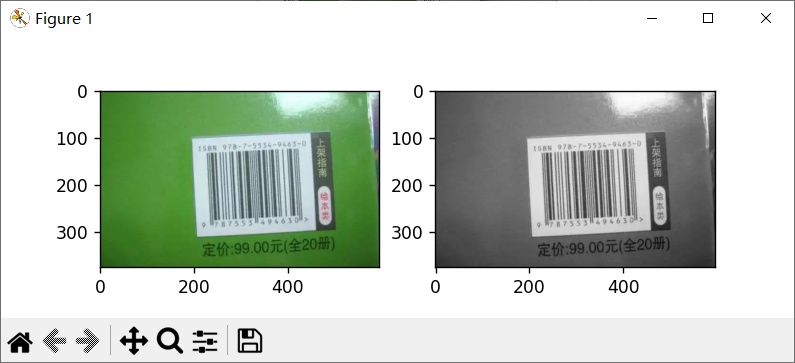
\includegraphics[height=120pt]{sample_toGrey}
    \caption{灰度化效果展示}
\end{figure}


\subsection{二值化}
根据课件(第9章-3基于阈值的图像分割)内容可知,可以按照图像的灰度不同,选取一个阈值 $x$,将灰度 $\ge x$ 的都转为一种灰度,其余的转为另一种灰度,实现二值化。这个阈值如果手动选取的话适应性不够强,所以考虑用基本自适应阈值。采用 Otsu 算法(最大类间方差法),具体步骤如下:
设图像长宽为 $n,m$,最佳阈值是 $x$,$< x$ 的点有 $n_0$ 个,$\ge x$ 的点有 $n_1$ 个,原图 $< x$ 的点平均灰度为 $\mu_0$,$\ge x$ 的点平均灰度为 $\mu_1$,令:
\[w_0=\frac{n_0}{nm},\quad w_1=\frac{n_1}{nm}\]
显然满足:
\[n_0+n_1=nm,\quad w_0+w_1=1\]
则二值化前的均值 $\mu$ 显然满足:
\[\mu=w_0\cdot\mu_0+w_1\cdot\mu_1\]
为了让方差最大化,设方差 $\sigma$ 为:
\[\sigma=w_0\cdot(\mu_0-\mu)^2+w_1\cdot(\mu_1-\mu)^2\]

联立解得:$\sigma=w_0\cdot w_1\cdot (\mu_0-\mu_1)^2$,因此,将所有 $\ge x$ 的点与 $< x$ 的点分别染色为两种灰度,即可实现灰度化。

具体到代码实现上,可以枚举 $x\in[0,255]$,然后分别计算 $\sigma$,将取得最大 $\sigma$ 的 $x$ 作为阈值即可。

考虑到在本题中,一般是从按的背景上分割出暗的物体(即数字),所以将 $< x$ 的都染为黑色,$\ge x$ 的都染成白色。

上述代码涉及大量遍历图像的操作,将其用\textbf{矩阵运算优化},能显著提升运算效率。时间复杂度为 $O(255nm)$,对较小的图像能以几乎一瞬间求出结果。

核心代码如下:
\begin{lstlisting}[language=python]
import numpy as np
def getThrestHold(img):
    n, m = img.shape
    mx, x = -1, 0  # mx是当前最大值,x是取得最值的阈值
    np.seterr(divide='ignore',invalid='ignore')#零除
    for i in range(0, 256):
        n0 = np.sum(img < i)
        n1 = n*m-n0
        w0 = n0/(n*m)
        w1 = 1-w0
        mu0 = np.sum(img[img < i])/n0
        mu1 = np.sum(img[img >= i])/n1
        g = w0*w1*(mu0-mu1)**2
        if g > mx:
            mx, x = g, i
    return x
def toBinary(img, x, ltx=0, gex=255):
    img2 = img.copy()
    img2[img2 < x] = ltx
    img2[img2 >= x] = gex
    return img2
\end{lstlisting}
运行效果如下:
\begin{figure}[htbp]
    \centering
    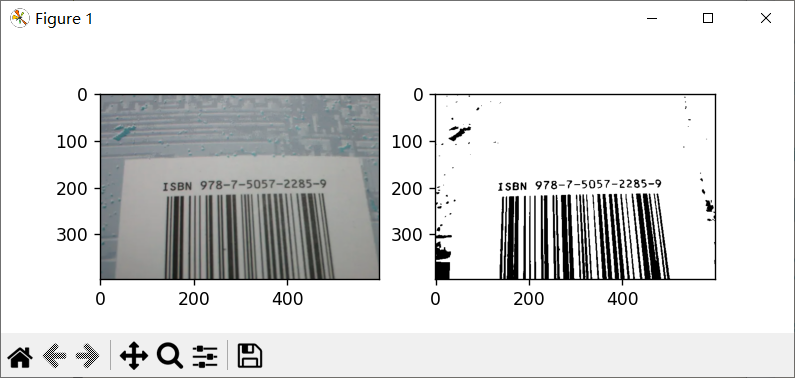
\includegraphics[height=120pt]{sample_toBinary}
    \caption{二值化效果展示}
\end{figure}


\subsection{字符定位及分割}
基本原理:将图片二值化之后(假设背景是白色,其余是黑色),在理想情况下(没有旋转、没有多余内容、噪声等),如果统计每一行每一列有多少个黑点,绘制水平和垂直统计图。核心代码如下:
\begin{lstlisting}[language=python]
def getHoriAndVertSum(img):
    img1 = ((255-img)//255).astype(np.uint16)
    sumVert = img1.sum(axis=0)
    sumHori = img1.sum(axis=1)
    return [sumHori, sumVert]
\end{lstlisting}
可以发现ISBN的部分会呈现出一段特殊波的形状,如图所示:\textit{(作图代码见附录)}
\begin{figure}[H]%让插入的图片紧跟在文字后面
    \centering
    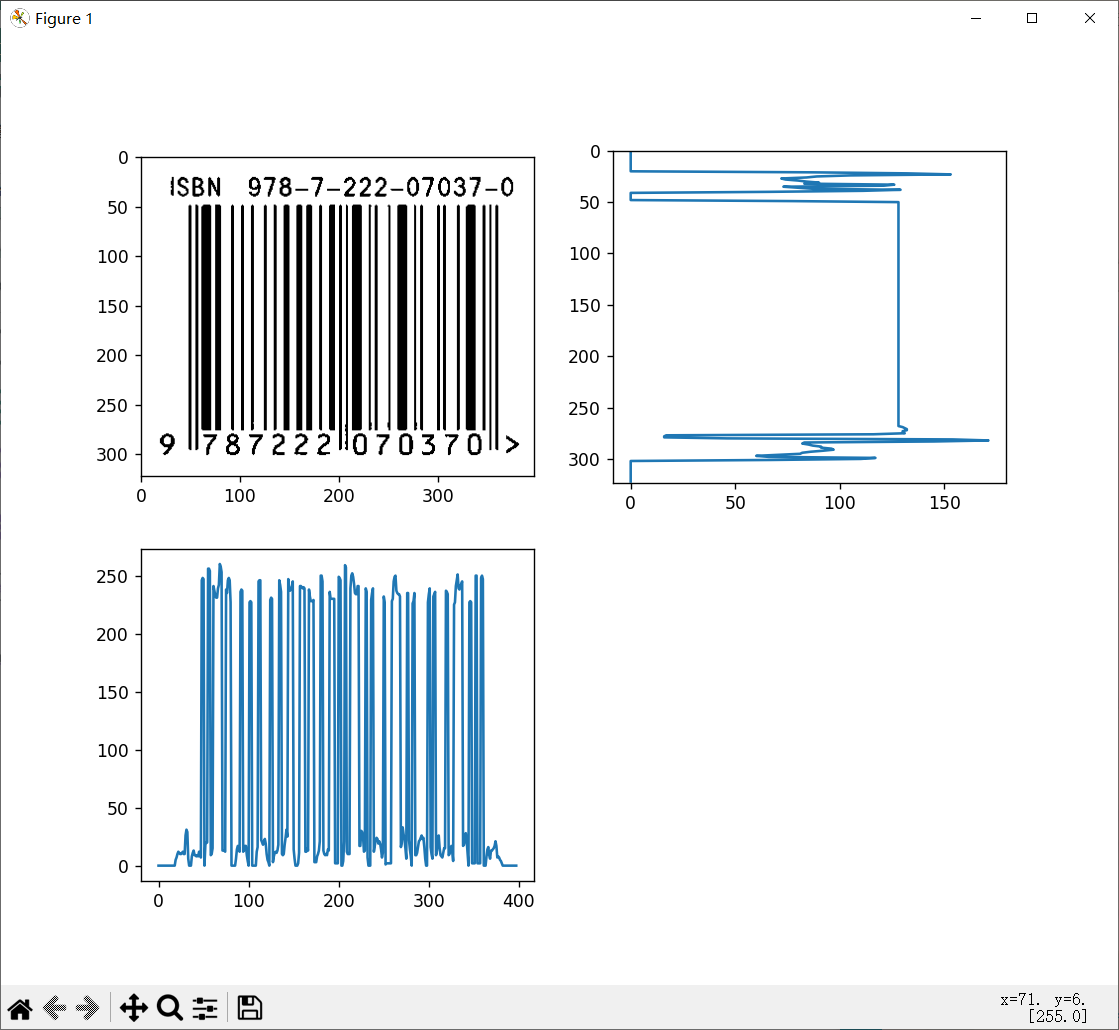
\includegraphics[height=260pt]{isbn_sum}
    \caption{ISBN图的统计特征}
\end{figure}

观察图像可知,垂直统计图的条形码处的波形波动也跟条形码一样剧烈变化,且水平统计图的条形码处是一段平的较高的图形。而ISBN号一定出现在其条形码的上下两端出现。根据ISBN号的知识可知,上下出现的数字一定是相同的。则任取一边进行识别即可。比较显然下方的数字更好处理,所以优先考虑识别下边的数字。

数字区域的水平特征是,出现在条形码区域的附近,且边界是低频率的。那么我们可以先按水平特征截取出数字行,再进一步分析。在实现上,可以设一个低频阈值 $low$,如果某一行出现黑点个数 $\ge low$,就开始记为边界,直到下一次再出现 $< low$ 的行就设为另一边界,并把边界之间的行全部提取出来。根据肉眼观察和经验推理,不妨预设 $low=25\%max$,即最高频次的 $25\%$。

核心代码如下:
\begin{lstlisting}[language=python]
def getNumberLineRange(sumHori, low=0.25):
    lim = np.max(sumHori)*low  # 实际阈值
    left, right = -1, -1
    n = sumHori.shape[0]
    for i in range(n-1, -1, -1):
        if sumHori[i] >= lim and right == -1:
            right = i
        if sumHori[i] < lim and right != -1:
            left = i
            break
    return [max(0, left), max(0, right)]
\end{lstlisting}

分割效果如下:
\begin{figure}[H]
    \centering
    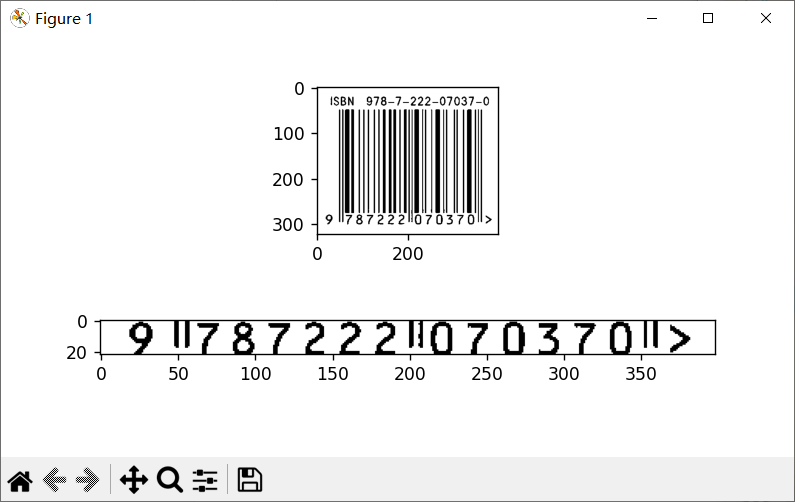
\includegraphics[height=120pt]{sample_splitRow}
    \caption{按行分割效果}
\end{figure}

将其按行分割后,再次求其列特征,调用上述函数,得到统计图如下:
\begin{figure}[H]
    \centering
    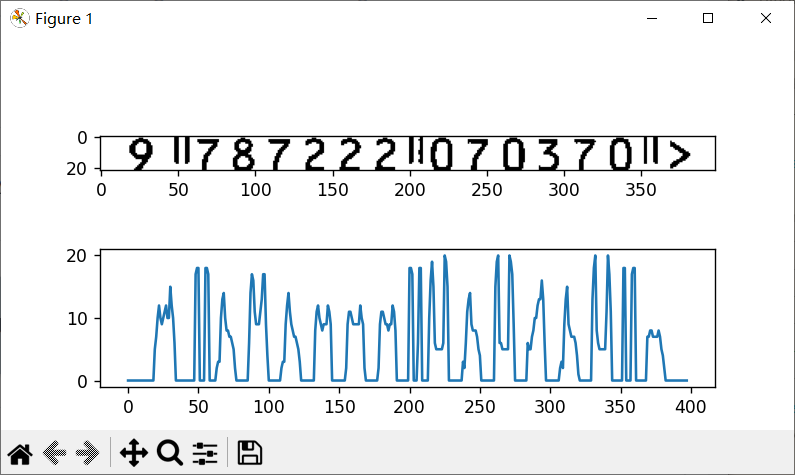
\includegraphics[height=120pt]{sample_splitRow_ana}
    \caption{按行分割后的按行统计图}
\end{figure}

可以发现,每个数字都对应一段连续的波。按照类似上面的办法将其分割即可。直接调整上述代码\textit{(见附录)},得到效果如下:
\begin{figure}[H]
    \centering
    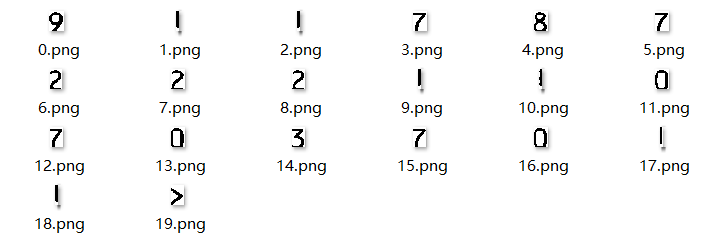
\includegraphics[height=100pt]{sample_splitNum}
    \caption{分割后得到的每个字符}
\end{figure}

可以发现,分割出来的内容里含有无关的元素,包括 ISBN 条形码的多余部分,还有 > 符号。对复杂的图像,可能还有一些噪声、误点等。考虑如何初步筛除这些内容。

关于图像去噪,可以用滤波器等方法先做预处理。对污点
考虑到ISBN里数字都是等大小的,我们可以取截取出来的长度中位数作为判定标准,如果某个区域明显比中位数小,例如不妨设比中位数的 $0.3$ 还要小,就把这个区域给删除掉。注意到在某些字体里,数字 $1$ 可能很小,这样有可能会误删数字 $1$。但是无论如何,条形码横线理论上会比数字 $1$ 更小。且如果是下面截断的 ISBN,条形码最多只有六条。也可以利用这个性质,最多只删除最短的六个区域,能够较大程度确保不会误删(但是有污点时可能少删)。对特殊符号 > 和其他元素的筛除,可能需要进行下一步计算匹配时再处理。

一种实现代码如下:
\begin{lstlisting}[language=python]
def filtRanges(arr, low=0.3, maxDel=6):
    n = len(arr)
    b = [(i, arr[i][1]-arr[i][0]) for i in range(n)]
    b.sort(key=lambda v: v[1])  # 按长度排序
    lim = low*b[n//2][1]  # 中位数
    ban = {b[i][0] for i in range(min(maxDel, n))
           if b[i][1] < lim}
    arr = [arr[i] for i in range(n) if i not in ban]
    return arr
\end{lstlisting}

效果如下,对条形码竖线效果显著:
\begin{figure}[H]
    \centering
    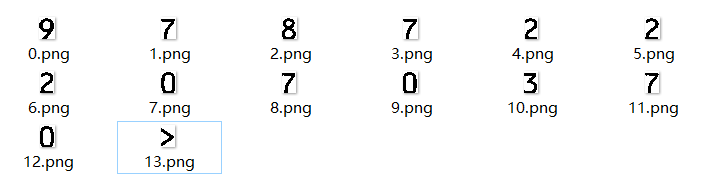
\includegraphics[height=85pt]{sample_splitNum_flit}
    \caption{分割后得到的每个字符(经初步筛查)}
\end{figure}

\subsection{预处理旋转}
上述字符定位与分割过程对理想状态的 ISBN 字符分割表现良好,但是并非所有图像都是理想的。最常见的就是存在旋转,如:

\begin{figure}[H]
    \centering
    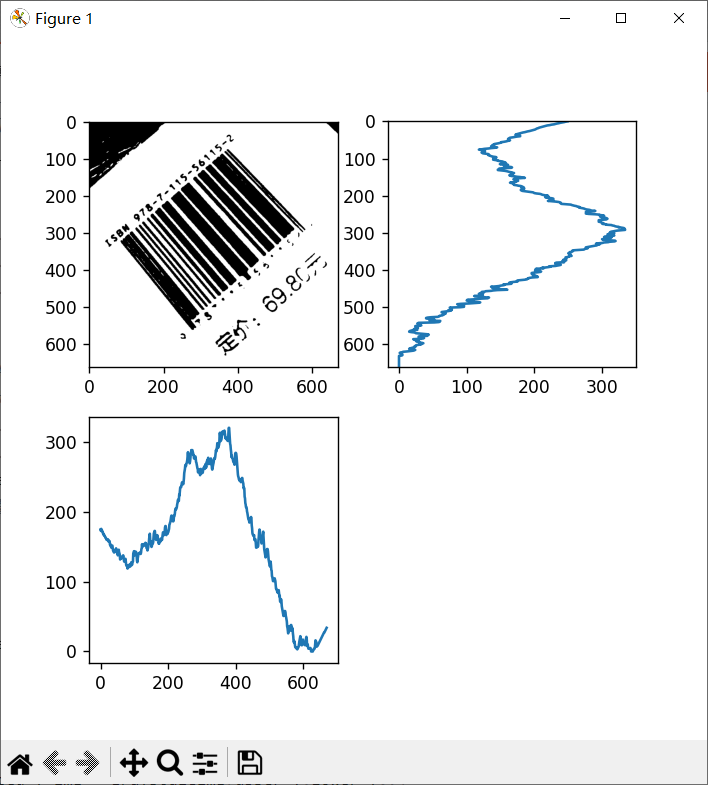
\includegraphics[height=260pt]{isbn_rotated}
    \caption{旋转过的ISBN图像及其分析}
\end{figure}

观察可知,ISBN 条形码明显的特征是有许多直线的条形,被旋转后,直线的朝向也会发生改变。如果我们能找出这些条形码直线及其旋转角,就能将其旋转回去。

根据课件(第9章-基于边缘检测的图像分割-Hough变换)可知,使用 Hough(霍夫)变换能够找到图中的直线。我们可以先使用 Canny 算子进行边缘检测,然后使用 Hough 变换对边缘检测结果提取其中的直线。

在实践过程中,不难发现,使用 Hough 变换需要设定一个阈值 $lim$,只有直线上的点数(即直线长度)超过 $lim$ 的直线才能被检测到。然而,图像变化多样,我们很难实现设定固定的 $lim$ 来满足不同的真实情境。因此,我采用了\textbf{倍增法}来快速枚举 $lim$ 的值,具体思想为:先设定一个较高的初始 $lim$,然后进行 Hough 变换找直线,如果找到的直线数目没有或很少,就证明阈值过高,这时将阈值除以一个常数来缩小阈值 $lim$,并继续查找,一直重复如上步骤直到找到为止。可以证明当阈值趋于 $0$ 时必然能找到。该算法能在对数复杂度内找到一个较为合适的阈值并进行直线分割。

核心代码如下:

\begin{lstlisting}[language=python]
def getLines(img):
    #传入二值化图像,输出其倍增法所有检测出来的直线
    #50,150是最小最大阈值,3是sobel卷积核大小
    edges = cv2.Canny(img, 50, 150, apertureSize=3)
    lim = int(np.min(img.shape)*0.8)
    while True:
        lines=cv2.HoughLines(edges,1,np.pi/180,lim)
        if type(lines) == type(None) 
            or len(lines) <= 5:
            lim = int(lim*0.9)
            continue#找不到/太少就不断缩小要求
        break
\end{lstlisting}

效果如图所示:

\begin{figure}[H]
    \centering
    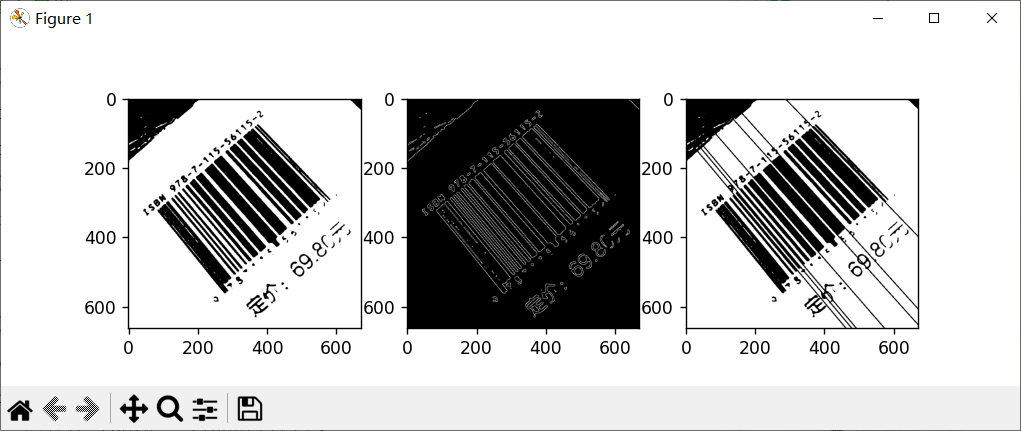
\includegraphics[height=120pt]{hough}
    \caption{Hough变换处理旋转图像提取直线并标注}
\end{figure}

进行上述过程后,实际上我们将得到一组直线。由于检测出来的直线不保证都是条形码上的直线,所以我们考虑选择这些直线里斜率处于中位数的作为图像的倾斜角,并对图像进行旋转还原。

Hough 变换得到的每条直线都是极坐标系下的 $(\rho,\theta)$ 参数,通过极坐标变换,可以计算出该直线在平面直角坐标下的任意两点,从而计算出直线的斜率。然后将直线斜率旋转到与纵坐标轴垂直即可。

代码如下:
\begin{lstlisting}[language=python]
def getMidAngle(lines):
    '''给定极坐标直线组,返回位于中位数斜角(角度制)'''
    lt = []
    for line in lines:
        rho, theta = line[0]
        a = np.cos(theta)
        b = np.sin(theta)
        x0 = a * rho
        y0 = b * rho
        x1 = int(x0 + 1000 * (-b))
        y1 = int(y0 + 1000 * (a))
        x2 = int(x0 - 1000 * (-b))
        y2 = int(y0 - 1000 * (a))
        k = np.arctan2(x2-x1, y2-y1)
        lt.append(k/np.pi*180)
    lt.sort()
    return lt[lines.shape[0]//2]
\end{lstlisting}

旋转时会产生新的图像区域,如果图片(书封面)本身是深色背景的,则图片边缘都是黑色的,应当用黑色填充;否则,应当用白色填充,可以进行特判,取出现频率最高的颜色进行填充。

进行旋转的核心代码如下:
\begin{lstlisting}[language=python]
def rotateImg(img, ang):
    #以中心旋转图像,顺时针转动ang角度并返回(白色填充)
    h, w = img.shape
    cx, cy = w//2, h//2
    # 1.0表示不缩放
    m = cv2.getRotationMatrix2D((cx, cy), -ang, 1.0)
    mc, ms = np.abs(m[0, 0:2])
    nw = int(h*ms+w*mc)
    nh = int(h*mc+w*ms)
    m[0, 2] += (nw/2)-cx
    m[1, 2] += (nh/2)-cy
    #分类讨论填充新区域的颜色
    numBlack = img[img == 0].size
    numWhite = img.size-numBlack
    if numBlack > numWhite:
        c = (0, 0, 0)
    else:
        c = (255, 255, 255)
    return cv2.warpAffine(img, m, (nw, nh),
            borderValue=c)
\end{lstlisting}

合并代码如下:
\begin{lstlisting}[language=python]
def autoRotate(img):
    '''以二值化图像为输入,输出自动旋转后的图像'''
    lines = getLines(img)
    ang = getMidAngle(lines)
    return rotateImg(img, ang)
\end{lstlisting}

效果图展示:
\begin{figure}[H]
    \centering
    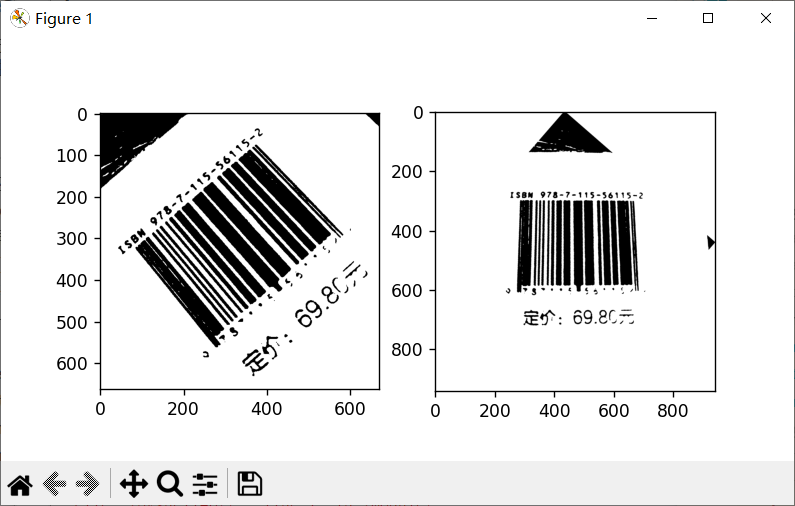
\includegraphics[height=120pt]{sample_autoRotate}
    \caption{将条形码自动旋转到垂直效果}
\end{figure}

显然,根据算法步骤可知,我们可以将条形码从“打横”的变成“打竖”的,但是旋转到大致垂直后,条形码上的字究竟是正的,还是反的,这是 Hough 变换无法实现的。为了解决这个问题,我们将在后续处理中,将图片分别当成是正的和反的都处理一遍,哪个匹配出更多内容就取哪个。

\subsection{预处理图片分割}
进行过预处理旋转后,仍有一个问题,如果图像不只有条形码,还有书本封面的其他内容,会干扰条形码的分析。所以我们希望能先预处理,使其只截取出条形码部分(如图3所示效果)。否则,其统计特征如下,进行分析困难:
\begin{figure}[H]
    \centering
    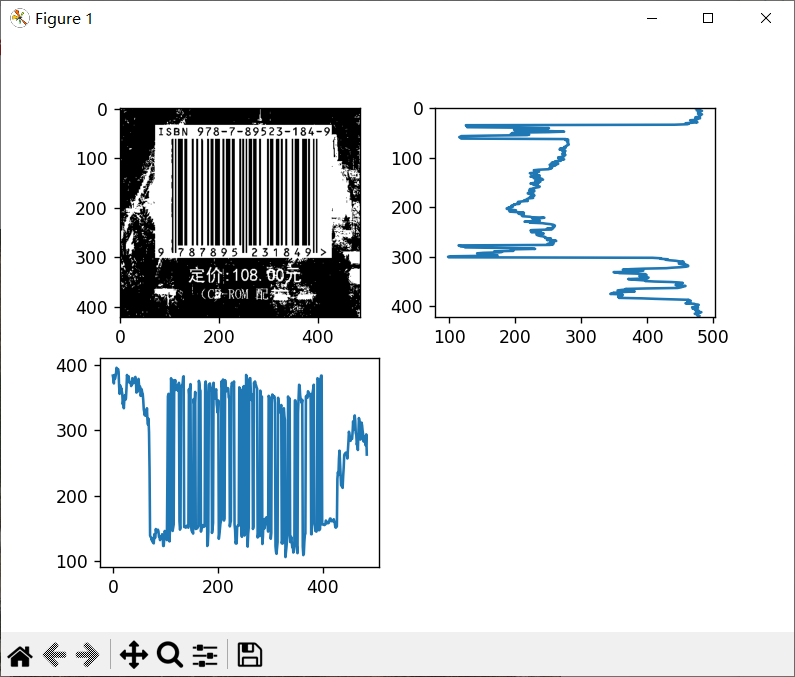
\includegraphics[height=120pt]{isbn_beforeCut}
    \caption{条形码外的封面内容干扰统计}
\end{figure}

\begin{comment}
根据课件(第12章-形态学图像处理)可知,数学形态学图像处理的基本思想是:用具有一定形态的结构元素(如一定大小的矩形、圆或菱形等)探测目标图像,能达到图像分析与识别的目的。因此,考虑使用形态学方法进行处理并提取出有效的子图区域。

观察可知,ISBN 的有效区域总是一个白色的矩形为背景的。我们可以考虑找到这个矩形区域并将其提取出来。

根据课件内容可知,闭运算(先膨胀再腐蚀)能磨光物体内边界,开运算(先腐蚀再膨胀)能磨光图像外边界。

根据类似的经验,我们可以先膨胀图像,将条形码矩形的内部内容去掉,用背景色替代,再进行一次腐蚀去噪。

不妨定义一个横向的长条矩形,如 $(n\times 1)$ 矩形进行膨胀;然后用 $(1\times m)$ 的纵向矩形进行腐蚀,去掉纵向的残留条形码等内容。考虑到膨胀与腐蚀操作的本质,我们认为 $n,m$ 的选取可以与具体图片的大小无关。这里使用的并非闭运算,因为前后不是同一个结构元素。根据经验,不妨设 $n=20,m=15$,实践表明,能取得较优的效果。

代码如下:
这是一段多行注释。
它可以包含任意多行文本。
注释内容不会在编译后的文档中显示。
\end{comment}

检测一张图像中出现的矩形区域,可以采用 这篇论文 中提出的算法。调用相关算法后,我们能够得到图像上的所有轮廓。根据本题的特殊性,我们只需要选取其中的所有矩形轮廓。特别地,有时候如果轮廓检测失败,可能会得到许多很小的轮廓,不妨设置一个阈值如 $20\%$,所有面积小于原图像的 $20\%$ 的矩形全部忽略掉。然后,我们取出最大的矩形,作为检测的目标。

为了得到更准确的结果,我们需要实现进行预处理,例如可以先进行高斯模糊,然后再用 Canny 算法做边缘检测,以边缘检测结果的二值化图像开始提取轮廓。

核心代码如下:

\begin{lstlisting}[language=python]
def getMainRectangle(img):
    '''传入任意图像,返回其出现的最大矩形区域'''
    imgGray = toGrey(img)
    # 高斯模糊
    imgBlur = cv2.GaussianBlur(imgGray, (5, 5), 1)
    # Canny算子边缘检测
    imgCanny = cv2.Canny(imgBlur, 60, 60)
    # 边缘检测,RETR_TREE可能更精准
    contours, _ = cv2.findContours(
    imgCanny, cv2.RETR_TREE, cv2.CHAIN_APPROX_NONE)
    res = []  # 答案
    nh, nw = img.shape[:2]
    totArea = nh*nw
    for obj in contours:
        # 计算轮廓内区域的面积
        area = cv2.contourArea(obj)
        if area <= 0.2*totArea:  # 矩形太小
            continue
        # 计算轮廓周长
        perimeter = cv2.arcLength(obj, True)
        # 获取轮廓角点坐标
        approx = cv2.approxPolyDP(
            obj, 0.02*perimeter, True)
        CornerNum = len(approx)  # 轮廓角点的数量
        # 获取坐标值和宽度、高度
        x, y, w, h = cv2.boundingRect(approx)
        if CornerNum == 4:  # 是矩形
            res.append([x, y, w, h])
    if len(res) == 0:  # 找不到
        return [0, 0, nw, nh]
    # 取出最大的矩形
    ans = max(res, key=lambda x: x[2]*x[3])  
    return ans
\end{lstlisting}

效果如图所示:

\begin{figure}[H]
    \centering
    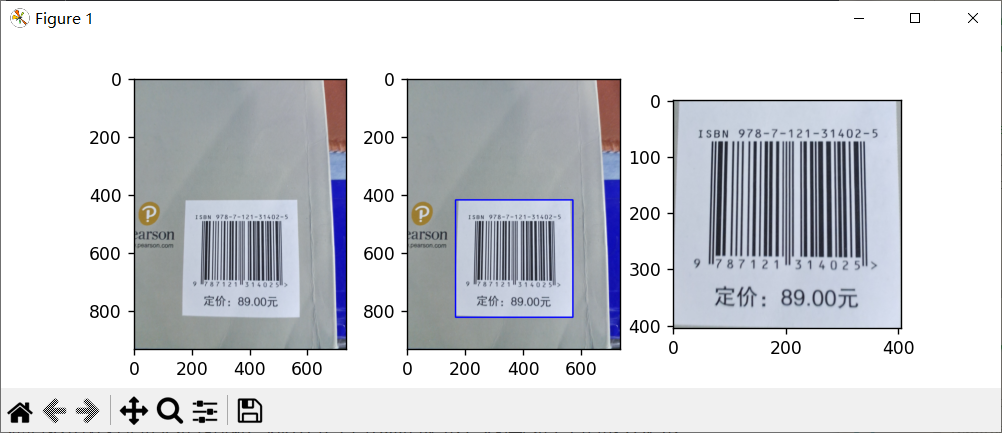
\includegraphics[height=120pt]{sample_graphSplit}
    \caption{截取图片中的矩形}
\end{figure}

然而,根据实践经验,直接进行矩形探测会有如下问题:如果书籍封面太花,即图案等干扰因素较多(如本节第一张图片)。为了达到更好的效果,我们可以进行两次分割。第一次分割直接调用上述做法,对第一次分割后的图像,再进行灰度化、二值化后进行第二次分割,以期望达到更好的效果。

如图所示(中图为第一次分割(找不到矩形),右图为第二次分割):

\begin{figure}[H]
    \centering
    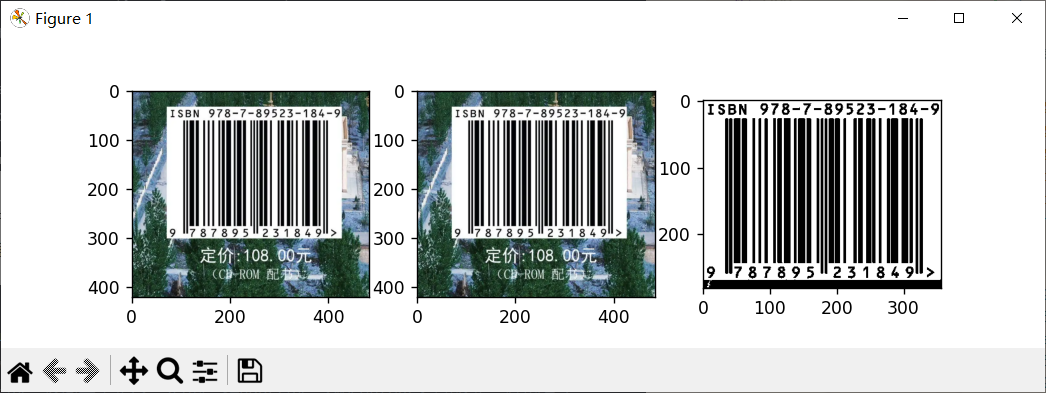
\includegraphics[height=120pt]{sample_graphSplit2}
    \caption{两次探测截取图片中的矩形}
\end{figure}

\section{实验结果及分析}
\section{总结与体会}
\section{致谢}
\section{参考文献}
Otsu 算法解析
%https://blog.csdn.net/a15779627836/article/details/124151125

数字分割
%https://www.cnblogs.com/skyfsm/p/8029668.html

Canny边缘检测
%https://blog.csdn.net/weixin_42272768/article/details/111244896

Hough变换详解
%https://blog.csdn.net/qq_30460949/article/details/90293147
%https://blog.csdn.net/qq_41112170/article/details/125729100

图片旋转
%https://blog.csdn.net/wyx100/article/details/80541726

提取特定图片区域
%https://blog.csdn.net/weixin_47365088/article/details/116566822

形状识别
%https://blog.csdn.net/LPYchengxuyuan/article/details/122003702?utm_medium=distribute.pc_relevant.none-task-blog-2~default~baidujs_baidulandingword~default-0-122003702-blog-124125975.pc_relevant_aa&spm=1001.2101.3001.4242.1&utm_relevant_index=3

边缘检测
%Suzuki, S. and Abe, K., TopologicalStructural Analysis of Digitized Binary Images by Border Following.CVGIP 30 1, pp32-46 (1985)

\section{附录}
\end{document}